\documentclass[12pt]{article}
\usepackage{titlesec}
\usepackage[dvipsnames]{xcolor}
\usepackage{tikz}
\usepackage{enumitem}
\usepackage{float}
\usepackage[usestackEOL]{stackengine}
\usepackage{scalerel}
\usepackage{graphicx,amsmath}
\usepackage{bbm}
\usepackage{amssymb}
\usepackage{cancel}
\usepackage{hyperref}
% Particle physics review, leo
\usetikzlibrary{shapes.geometric, arrows,positioning}
\usepackage[utf8]{inputenc}
\usepackage{pgfplots}
\usepackage{booktabs}
\usepackage{physics}
\usepackage{cancel}
\usepackage{wasysym}
\usepackage{fancyvrb}
\usepackage{enumerate}

\title{Alpha Zero Symbolic Regression Algorithm}
\pgfplotsset{compat=1.18}

\tikzset{snake it/.style={decorate, decoration=snake}}
\usetikzlibrary{intersections, pgfplots.fillbetween, decorations.pathmorphing,decorations.shapes,decorations.markings}

\definecolor{gold}{RGB}{218,165,32}
\definecolor{grassgreen}{RGB}{0,128,0}
\definecolor{purple}{RGB}{128,0,128}
\titleformat*{\section}{\huge\bfseries}
\titleformat*{\subsection}{\LARGE\bfseries}
\titleformat*{\subsubsection}{\Large\bfseries}

\parskip \baselineskip
\def\myupbracefill#1{\rotatebox{90}{\stretchto{\{}{#1}}}
\def\mydownbracefill#1{\rotatebox{270}{\stretchto{\{}{#1}}}
\def\rlwd{.5pt}

\newcommand\notate[4][B]{%
  \if B#1\else\def\myupbracefill##1{}\fi%
  \def\useanchorwidth{T}%
  \setbox0=\hbox{$\displaystyle#2$}%
  \def\stackalignment{c}\stackunder[-7.425pt]{%
    \def\stackalignment{c}\stackunder[-1.5pt]{%
      \stackunder[-2pt]{\strut $\displaystyle#2$}{}}{%
    \rule{\rlwd}{#3\baselineskip}}}{%
  \strut\kern9pt$\hspace{.055cm}\rightarrow$\smash{\rlap{$~\displaystyle#4$}}}%
}

\newcommand\linelessnotate[4][B]{%
%   \if B#1\else\def\myupbracefill##1{}\fi%
%   \def\useanchorwidth{T}%
%   \setbox0=\hbox{$\displaystyle#2$}%
  \def\stackalignment{c}\stackunder[-15pt]{%
    \def\stackalignment{c}\stackunder[0pt]{%
      \stackunder[0pt]{\strut $\displaystyle#2$}{}}{%
    \rule{0 pt}{#3\baselineskip}}}{%
  \strut\kern9pt$\hspace{.108cm}$\smash{\rlap{$~\displaystyle#4$}}}%
}

\newcommand\notateone[4][B]{%
  \if B#1\else\def\myupbracefill##1{}\fi%
  \def\useanchorwidth{T}%
  \setbox0=\hbox{$\displaystyle#2$}%
  \def\stackalignment{c}\stackunder[-7.425pt]{%
    \def\stackalignment{c}\stackunder[3.5pt]{%
      \stackunder[-2pt]{\strut $\displaystyle#2$}{}}{%
    \rule{\rlwd}{#3\baselineskip}}}{%
  \strut\kern9pt$\hspace{.055cm}\rightarrow$\smash{\rlap{$~\displaystyle#4$}}}%
}

\newcommand\notategreen[4][B]{%
  \if B#1\else\def\myupbracefill##1{}\fi%
  \def\useanchorwidth{T}%
  \setbox0=\hbox{$\displaystyle#2$}%
  \def\stackalignment{c}\stackunder[-9.5pt]{%
    \def\stackalignment{c}\color{green}\stackunder[-.5pt]{%
      \stackunder[-2pt]{\strut $\displaystyle#2$}{}}{
    \rule{\rlwd}{#3\baselineskip}}}{%
  \strut\kern9pt$\hspace{.108cm}\color{green}\rightarrow$\smash{\rlap{$~\displaystyle#4$}}}%
}

\newcommand\invnotate[4][B]{%
  \if B#1\else\def\myupbracefill##1{}\fi%
  \def\useanchorwidth{T}%
  \setbox0=\hbox{$\displaystyle#2$}%
  \def\stackalignment{c}\stackon[-9.5pt]{%
    \def\stackalignment{c}\stackon[.5pt]{%
      \stackon[-2pt]{\strut $\displaystyle#2$}{}}{%
    \rule{\rlwd}{#3\baselineskip}}}{%
  \strut\kern9pt$\hspace{.108cm}\rightarrow$\smash{\rlap{$~\displaystyle#4$}}}%
}

\newcommand\invnotatelow[4][B]{%
  \if B#1\else\def\myupbracefill##1{}\fi%
  \def\useanchorwidth{T}%
  \setbox0=\hbox{$\displaystyle#2$}%
  \def\stackalignment{c}\stackon[-9.5pt]{%
    \def\stackalignment{c}\stackon[-3.5pt]{% controls how much above it is
      \stackon[-2pt]{\strut $\displaystyle#2$}{}}{%
    \rule{\rlwd}{#3\baselineskip}}}{%
  \strut\kern9pt$\hspace{.108cm}\rightarrow$\smash{\rlap{$~\displaystyle#4$}}}%
}

\newcommand\invnotateone[4][B]{%
  \if B#1\else\def\myupbracefill##1{}\fi%
  \def\useanchorwidth{T}%
  \setbox0=\hbox{$\displaystyle#2$}%
  \def\stackalignment{c}\stackon[-9.5pt]{%
    \def\stackalignment{c}\stackon[3.5pt]{%
      \stackon[-2pt]{\strut $\displaystyle#2$}{}}{%
    \rule{\rlwd}{#3\baselineskip}}}{%
  \strut\kern9pt$\hspace{.108cm}\rightarrow$\smash{\rlap{$~\displaystyle#4$}}}%
}

\newcommand\invnotatetwo[4][B]{%
  \if B#1\else\def\myupbracefill##1{}\fi%
  \def\useanchorwidth{T}%
  \setbox0=\hbox{$\displaystyle#2$}%
  \def\stackalignment{c}\stackon[-9.5pt]{%
    \def\stackalignment{c}\stackon[-20pt]{%
      \stackon[-2pt]{\strut $\displaystyle#2$}{}}{%
    \rule{\rlwd}{#3\baselineskip}}}{%
  \strut\kern9pt$\hspace{.108cm}\rightarrow$\smash{\rlap{$~\displaystyle#4$}}}%
}

\newcommand\invnotatemagenta[4][B]{%
  \if B#1\else\def\myupbracefill##1{}\fi%
  \def\useanchorwidth{T}%
  \setbox0=\hbox{$\displaystyle#2$}%
  \def\stackalignment{c}\stackon[-9.5pt]{%
    \def\stackalignment{c}\color{magenta}\stackon[0pt]{%
      \stackon[-2pt]{\strut $\displaystyle#2$}{}}{%
    \rule{\rlwd}{#3\baselineskip}}}{%
  \strut\kern9pt$\hspace{.108cm}\color{magenta}\rightarrow$\smash{\rlap{$~\displaystyle#4$}}}%
}


\newcommand\curlnotate[4][B]{%
  \if B#1\else\def\myupbracefill##1{}\fi%
  \def\useanchorwidth{T}%
  \setbox0=\hbox{$\displaystyle#2$}%
  \def\stackalignment{c}\stackunder[-7.43pt]{%
    \def\stackalignment{c}\stackunder[-1.5pt]{%
      \stackunder[2pt]{\strut $\displaystyle#2$}{\myupbracefill{\wd0}}}{%
    \rule{\rlwd}{#3\baselineskip}}}{%
  \strut\kern9pt$\hspace{.06cm}\rightarrow$\smash{\rlap{$~\displaystyle#4$}}}%
}

\newcommand\curlnotateone[4][B]{%
  \if B#1\else\def\myupbracefill##1{}\fi%
  \def\useanchorwidth{T}%
  \setbox0=\hbox{$\displaystyle#2$}%
  \def\stackalignment{c}\stackunder[-9.5pt]{%
    \def\stackalignment{c}\stackunder[-3.5pt]{%
      \stackunder[7pt]{\strut $\displaystyle#2$}{\myupbracefill{\wd0}}}{%
    \rule{\rlwd}{#3\baselineskip}}}{%
  \strut\kern9pt$\hspace{.108cm}\rightarrow$\smash{\rlap{$~\displaystyle#4$}}}%
}


\newcommand\invcurlnotate[4][B]{%
  \if B#1\else\def\mydownbracefill##1{}\fi%
  \def\useanchorwidth{T}%
  \setbox0=\hbox{$\displaystyle#2$}%
  \def\stackalignment{c}\stackon[-7.6pt]{%
    \def\stackalignment{c}\stackon[-1.5pt]{%
      \stackon[2pt]{\strut $\displaystyle#2$}{\mydownbracefill{\wd0}}}{%
    \rule{\rlwd}{#3\baselineskip}}}{%
  \strut\kern9pt$\hspace{.067cm}\rightarrow$\smash{\rlap{$~\displaystyle#4$}}}%
}

\newcommand\invcurlnotateone[4][B]{%
  \if B#1\else\def\mydownbracefill##1{}\fi%
  \def\useanchorwidth{T}%
  \setbox0=\hbox{$\displaystyle#2$}%
  \def\stackalignment{c}\stackon[-9.5pt]{%
    \def\stackalignment{c}\stackon[-2.7pt]{%
      \stackon[-5pt]{\strut $\displaystyle#2$}{\mydownbracefill{\wd0}}}{%
    \rule{\rlwd}{#3\baselineskip}}}{%
  \strut\kern9pt$\hspace{.108cm}\rightarrow$\smash{\rlap{$~\displaystyle#4$}}}%
}

\makeatletter
\newcommand*{\encircled}[1]{\relax\ifmmode\mathpalette\@encircled@math{#1}\else\@encircled{#1}\fi}
\newcommand*{\@encircled@math}[2]{\@encircled{$\m@th#1#2$}}
\newcommand*{\@encircled}[1]{%
  \tikz[baseline,anchor=base]{\node[draw,circle,outer sep=0pt,inner sep=.2ex] {#1};}}
\makeatother


\makeatletter
\newcommand*{\encircledgreen}[1]{\relax\ifmmode\mathpalette\@encircledgreen@math{#1}\else\@encircledgreen{#1}\fi}
\newcommand*{\@encircledgreen@math}[2]{\@encircledgreen{$\m@th#1#2$}}
\newcommand*{\@encircledgreen}[1]{%
  \tikz[baseline,anchor=base]{\node[draw,circle,outer sep=0pt,inner sep=.2ex,green] {#1};}}
\makeatother

\makeatletter
\newcommand*{\encircledmagenta}[1]{\relax\ifmmode\mathpalette\@encircledmagenta@math{#1}\else\@encircledmagenta{#1}\fi}
\newcommand*{\@encircledmagenta@math}[2]{\@encircledmagenta{$\m@th#1#2$}}
\newcommand*{\@encircledmagenta}[1]{%
  \tikz[baseline,anchor=base]{\node[draw,circle,outer sep=0pt,inner sep=.2ex,magenta] {#1};}}
\makeatother


%https://www.overleaf.com/learn/latex/LaTeX_Graphics_using_TikZ%3A_A_Tutorial_for_Beginners_(Part_3)—Creating_Flowcharts
\tikzstyle{startstop} = [rectangle, rounded corners, minimum width=3cm, minimum height=1cm,text centered, draw=black, fill=red!30]
\tikzstyle{io} = [rectangle, rounded corners, minimum width=3cm, minimum height=1cm,text centered, draw=black, fill=blue!30]
\tikzstyle{process} = [rectangle, rounded corners, minimum width=3cm, minimum height=1cm,text centered, draw=black, fill=orange!30]
\tikzstyle{decision} = [rectangle, rounded corners, minimum width=3cm, minimum height=1cm,text centered, draw=black, fill=green!30]
\tikzstyle{na} = [text centered]

\tikzstyle{arrow} = [thick,->,>=stealth]
\tikzstyle{line} = [thick,-,>=stealth]

\newlist{redenum}{enumerate}{1}
\setlist[redenum,1]{
    label=\textcolor{red}{\textbf{\arabic*)}}
}

\newlist{goldenum}{enumerate}{1}
\setlist[goldenum,1]{
    label=\textcolor{gold}{\text{\arabic*.)}}
}

\newlist{redenumnest}{enumerate}{1}
\setlist[redenumnest,1]{
    label=\textcolor{red}{\text{\arabic*.)}}
}

\newlist{magentaenum}{enumerate}{1}
\setlist[magentaenum,1]{
    label=\textcolor{magenta}{\text{\arabic*.)}}
}

\newlist{grassgreenenum}{enumerate}{1}
\setlist[grassgreenenum,1]{
    label=\textcolor{grassgreen}{\text{\arabic*.)}}
}

\newlist{purpleenum}{enumerate}{1}
\setlist[purpleenum,1]{
    label=\textcolor{purple}{\text{\arabic*.)}}
}

\newlist{blueenum}{enumerate}{1}
\setlist[blueenum,1]{
    label=\textcolor{blue}{\text{\arabic*.)}}
}

\newlist{cyanenum}{enumerate}{1}
\setlist[cyanenum,1]{
    label=\textcolor{cyan}{\text{\arabic*.)}}
}

\newlist{brownenum}{enumerate}{1}
\setlist[brownenum,1]{
    label=\textcolor{brown}{\text{\arabic*.)}}
}

\setlistdepth{40}

\begin{document}

\maketitle
% re.sub("[*][{]\d+[.]*\d*[.]*\d*\s+","{",txt)
% \tableofcontents
\newpage

\begin{redenum}
    \item Create game object
    \begin{itemize}
	\item[--] \textbf{n} = length of desired expression 
	\item[--] $b$ = board of game
	\begin{itemize}
		\item[$\rightarrow$] \textbf{n} pieces (all 0 initially)
		\item[$\rightarrow$] possible initial moves
		\item[$\rightarrow$] legal moves stemming from all possible previous moves
	 \end{itemize}
    \end{itemize}
    \item Create neural network wrapper object from game object
    \begin{itemize}
	\item[--] Create symbolic regression neural network
	\begin{itemize}
		\item[$\rightarrow$] size of input board = \textbf{n}
		\item[$\rightarrow$] size of output = \# of tokens considered = \textbf{o}
		\item[$\rightarrow$] \textbf{NN} model, see below example for \textbf{n} = 3 and \textbf{o} = 7
		\begin{center}
  
\tiny
			\begin{BVerbatim}
__________________________________________________________________________________________________
 Layer (type)                   Output Shape         Param #     Connected to                     
==================================================================================================
 input_1 (InputLayer)           [(None, 3, 1)]       0           []                               
                                                                                                  
 conv1d (Conv1D)                (None, 3, 512)       2048        ['input_1[0][0]']                
                                                                                                  
 batch_normalization (BatchNorm  (None, 3, 512)      2048        ['conv1d[0][0]']                 
 alization)                                                                                       
                                                                                                  
 activation (Activation)        (None, 3, 512)       0           ['batch_normalization[0][0]']    
                                                                                                  
 conv1d_1 (Conv1D)              (None, 3, 512)       786944      ['activation[0][0]']             
                                                                                                  
 batch_normalization_1 (BatchNo  (None, 3, 512)      2048        ['conv1d_1[0][0]']               
 rmalization)                                                                                     
                                                                                                  
 activation_1 (Activation)      (None, 3, 512)       0           ['batch_normalization_1[0][0]']  
                                                                                                  
 conv1d_2 (Conv1D)              (None, 3, 512)       786944      ['activation_1[0][0]']           
                                                                                                  
 batch_normalization_2 (BatchNo  (None, 3, 512)      2048        ['conv1d_2[0][0]']               
 rmalization)                                                                                     
                                                                                                  
 activation_2 (Activation)      (None, 3, 512)       0           ['batch_normalization_2[0][0]']  
                                                                                                  
 conv1d_3 (Conv1D)              (None, 1, 512)       786944      ['activation_2[0][0]']           
                                                                                                  
 batch_normalization_3 (BatchNo  (None, 1, 512)      2048        ['conv1d_3[0][0]']               
 rmalization)                                                                                     
                                                                                                  
 activation_3 (Activation)      (None, 1, 512)       0           ['batch_normalization_3[0][0]']  
                                                                                                  
 flatten (Flatten)              (None, 512)          0           ['activation_3[0][0]']           
                                                                                                  
 dense (Dense)                  (None, 1024)         525312      ['flatten[0][0]']                
                                                                                                  
 batch_normalization_4 (BatchNo  (None, 1024)        4096        ['dense[0][0]']                  
 rmalization)                                                                                     
                                                                                                  
 activation_4 (Activation)      (None, 1024)         0           ['batch_normalization_4[0][0]']  
                                                                                                  
 dropout (Dropout)              (None, 1024)         0           ['activation_4[0][0]']           
                                                                                                  
 dense_1 (Dense)                (None, 512)          524800      ['dropout[0][0]']                
                                                                                                  
 batch_normalization_5 (BatchNo  (None, 512)         2048        ['dense_1[0][0]']                
 rmalization)                                                                                     
                                                                                                  
 activation_5 (Activation)      (None, 512)          0           ['batch_normalization_5[0][0]']  
                                                                                                  
 dropout_1 (Dropout)            (None, 512)          0           ['activation_5[0][0]']           
                                                                                                  
 pi (Dense)                     (None, 7)            3591        ['dropout_1[0][0]']              
                                                                                                  
 v (Dense)                      (None, 1)            513         ['dropout_1[0][0]']              
                                                                                                  
==================================================================================================
Total params: 3,431,432
Trainable params: 3,424,264
Non-trainable params: 7,168
__________________________________________________________________________________________________

			\end{BVerbatim}
		\end{center}
\begin{center}
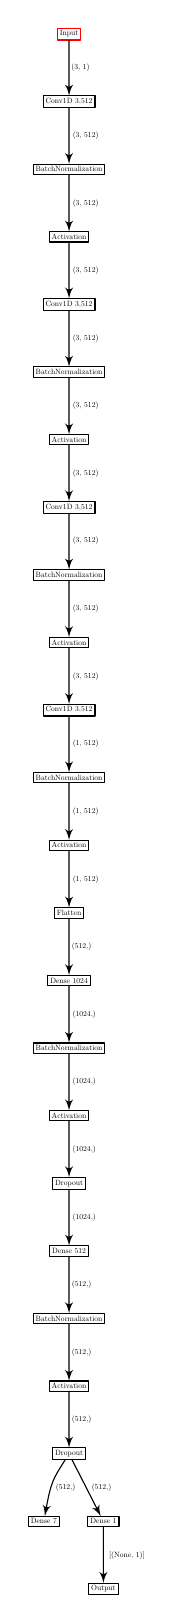
\begin{tikzpicture}[>=latex',line join=bevel,]
\begin{scope}[decoration={
    markings,
    mark=at position 1
    with {\arrow[scale=1.35]{stealth}}},scale=0.275, every node/.style={scale=0.275}] 
%%
\node (4749096464) at (63.125bp,2053.5bp) [draw=red,rectangle] {Input};
  \node (6360244960) at (63.125bp,1965.0bp) [draw,rectangle] {Conv1D 3,512};
  \node (6360245008) at (63.125bp,1876.5bp) [draw,rectangle] {BatchNormalization};
  \node (6358040480) at (63.125bp,1788.0bp) [draw,rectangle] {Activation};
  \node (6370543264) at (63.125bp,1699.5bp) [draw,rectangle] {Conv1D 3,512};
  \node (6370515552) at (63.125bp,1611.0bp) [draw,rectangle] {BatchNormalization};
  \node (6360246016) at (63.125bp,1522.5bp) [draw,rectangle] {Activation};
  \node (6370679968) at (63.125bp,1434.0bp) [draw,rectangle] {Conv1D 3,512};
  \node (6370678336) at (63.125bp,1345.5bp) [draw,rectangle] {BatchNormalization};
  \node (6370544032) at (63.125bp,1257.0bp) [draw,rectangle] {Activation};
  \node (6370802368) at (63.125bp,1168.5bp) [draw,rectangle] {Conv1D 3,512};
  \node (6370802704) at (63.125bp,1080.0bp) [draw,rectangle] {BatchNormalization};
  \node (6370801504) at (63.125bp,991.5bp) [draw,rectangle] {Activation};
  \node (6370803376) at (63.125bp,903.0bp) [draw,rectangle] {Flatten};
  \node (6360858688) at (63.125bp,814.5bp) [draw,rectangle] {Dense 1024};
  \node (6360858784) at (63.125bp,726.0bp) [draw,rectangle] {BatchNormalization};
  \node (6370514016) at (63.125bp,637.5bp) [draw,rectangle] {Activation};
  \node (6370680112) at (63.125bp,549.0bp) [draw,rectangle] {Dropout};
  \node (6370881104) at (63.125bp,460.5bp) [draw,rectangle] {Dense 512};
  \node (6370881392) at (63.125bp,372.0bp) [draw,rectangle] {BatchNormalization};
  \node (6370848832) at (63.125bp,283.5bp) [draw,rectangle] {Activation};
  \node (6361147232) at (63.125bp,195.0bp) [draw,rectangle] {Dropout};
  \node (6370929248) at (30.125bp,106.5bp) [draw,rectangle] {Dense 7};
  \node (6372247920) at (108.12bp,106.5bp) [draw,rectangle] {Dense 1};
  \node (output_node) at (108.12bp,18.0bp) [draw,rectangle] {Output};
  \draw [->] (4749096464) ..controls (63.125bp,2023.6bp) and (63.125bp,2007.7bp)  .. (6360244960);
  \definecolor{strokecol}{rgb}{0.0,0.0,0.0};
  \pgfsetstrokecolor{strokecol}
  \draw (78.125bp,2009.2bp) node {(3, 1)};
  \draw [->] (6360244960) ..controls (63.125bp,1935.1bp) and (63.125bp,1919.2bp)  .. (6360245008);
  \draw (84.875bp,1920.8bp) node {(3, 512)};
  \draw [->] (6360245008) ..controls (63.125bp,1846.6bp) and (63.125bp,1830.7bp)  .. (6358040480);
  \draw (84.875bp,1832.2bp) node {(3, 512)};
  \draw [->] (6358040480) ..controls (63.125bp,1758.1bp) and (63.125bp,1742.2bp)  .. (6370543264);
  \draw (84.875bp,1743.8bp) node {(3, 512)};
  \draw [->] (6370543264) ..controls (63.125bp,1669.6bp) and (63.125bp,1653.7bp)  .. (6370515552);
  \draw (84.875bp,1655.2bp) node {(3, 512)};
  \draw [->] (6370515552) ..controls (63.125bp,1581.1bp) and (63.125bp,1565.2bp)  .. (6360246016);
  \draw (84.875bp,1566.8bp) node {(3, 512)};
  \draw [->] (6360246016) ..controls (63.125bp,1492.6bp) and (63.125bp,1476.7bp)  .. (6370679968);
  \draw (84.875bp,1478.2bp) node {(3, 512)};
  \draw [->] (6370679968) ..controls (63.125bp,1404.1bp) and (63.125bp,1388.2bp)  .. (6370678336);
  \draw (84.875bp,1389.8bp) node {(3, 512)};
  \draw [->] (6370678336) ..controls (63.125bp,1315.6bp) and (63.125bp,1299.7bp)  .. (6370544032);
  \draw (84.875bp,1301.2bp) node {(3, 512)};
  \draw [->] (6370544032) ..controls (63.125bp,1227.1bp) and (63.125bp,1211.2bp)  .. (6370802368);
  \draw (84.875bp,1212.8bp) node {(3, 512)};
  \draw [->] (6370802368) ..controls (63.125bp,1138.6bp) and (63.125bp,1122.7bp)  .. (6370802704);
  \draw (84.875bp,1124.2bp) node {(1, 512)};
  \draw [->] (6370802704) ..controls (63.125bp,1050.1bp) and (63.125bp,1034.2bp)  .. (6370801504);
  \draw (84.875bp,1035.8bp) node {(1, 512)};
  \draw [->] (6370801504) ..controls (63.125bp,961.64bp) and (63.125bp,945.73bp)  .. (6370803376);
  \draw (84.875bp,947.25bp) node {(1, 512)};
  \draw [->] (6370803376) ..controls (63.125bp,873.14bp) and (63.125bp,857.23bp)  .. (6360858688);
  \draw (79.625bp,858.75bp) node {(512,)};
  \draw [->] (6360858688) ..controls (63.125bp,784.64bp) and (63.125bp,768.73bp)  .. (6360858784);
  \draw (83.0bp,770.25bp) node {(1024,)};
  \draw [->] (6360858784) ..controls (63.125bp,696.14bp) and (63.125bp,680.23bp)  .. (6370514016);
  \draw (83.0bp,681.75bp) node {(1024,)};
  \draw [->] (6370514016) ..controls (63.125bp,607.64bp) and (63.125bp,591.73bp)  .. (6370680112);
  \draw (83.0bp,593.25bp) node {(1024,)};
  \draw [->] (6370680112) ..controls (63.125bp,519.14bp) and (63.125bp,503.23bp)  .. (6370881104);
  \draw (83.0bp,504.75bp) node {(1024,)};
  \draw [->] (6370881104) ..controls (63.125bp,430.64bp) and (63.125bp,414.73bp)  .. (6370881392);
  \draw (79.625bp,416.25bp) node {(512,)};
  \draw [->] (6370881392) ..controls (63.125bp,342.14bp) and (63.125bp,326.23bp)  .. (6370848832);
  \draw (79.625bp,327.75bp) node {(512,)};
  \draw [->] (6370848832) ..controls (63.125bp,253.64bp) and (63.125bp,237.73bp)  .. (6361147232);
  \draw (79.625bp,239.25bp) node {(512,)};
  \draw [->] (6361147232) ..controls (47.972bp,171.26bp) and (44.571bp,165.04bp)  .. (42.125bp,159.0bp) .. controls (39.081bp,151.48bp) and (36.709bp,143.02bp)  .. (6370929248);
  \draw (58.625bp,150.75bp) node {(512,)};
  \draw [->] (6361147232) ..controls (78.323bp,164.79bp) and (86.915bp,148.27bp)  .. (6372247920);
  \draw (105.62bp,150.75bp) node {(512,)};
  \draw [->] (6372247920) ..controls (108.12bp,76.64bp) and (108.12bp,60.729bp)  .. (output_node);
  \draw (138.88bp,62.25bp) node {[(None, 1)]};
%
\end{scope}
\end{tikzpicture}

% End of code
\end{center}
    	\end{itemize}
    \end{itemize}

\item Create coach object, responsible for executing self.play + learning
	\begin{itemize}
	\item[--] Game Object \textcolor{red}{\textbf{(1)}}
	\item[--] Neural Network Object \textcolor{red}{\textbf{(2)}}
	\item[--] Arguments
		\begin{itemize}
			\item[$\rightarrow$] \# of iterations
			\item[$\rightarrow$] \# of episodes per iteration
			\item[$\rightarrow$] \# of training examples $\left(\text{of the form } \left[p_i, v, r\right]\right)$
			\item[$\rightarrow$] \# of arena games to determine if new neural network will be accepted
		\end{itemize}
	\item[--] MCTS object
		\begin{itemize}
			\item[$\rightarrow$] Game Object \textcolor{red}{\textbf{(1)}}
			\item[$\rightarrow$] Neural Network Object \textcolor{red}{\textbf{(2)}}
			\item[$\rightarrow$] Arguments (same as above)
			\item[$\rightarrow$]  Dictionaries (all initially empty)
			\begin{itemize}
				\item $Q(s,a)$: Average value of cumulative rewards received after taking action $a$ from state $s$; agent's current (at state $s$) estimate of action $a$'s expected value
				\item $N(s,a)$: visit counts for action $a$ at state $s$
				\item $N(s)$: visit counts for state $s$
				\item $P(s)$: estimated vector of prior probabilities of taking actions $\left(a_1, a_2, \ldots, a_{\textbf{o}} \right)$ from state $s$ (estimated initially by neural network)
				\item $E(s)$: stores end state for state $s$ (-1 = not finished, $0 \leq E(s) \leq 1$ = finished score (0 is the worst possible score and 1 is the best possible score))
				\item $V(s)$: vector of 1's and 0's of size \textbf{o} representing if token $i$ $(0, 1, \ldots,\textbf{o}-1)$ is valid (1) or not (0)
			
			\end{itemize}
		\end{itemize}
	\item[--] trainExampleHistory (initially empty): list of deques of training examples for 1 episode of the form $\left[s_i, p_i, r\right]$
		\begin{itemize}
			\item[$\rightarrow$] $s_i$: state (expression list in our case)
			\item[$\rightarrow$] $p_i$: policy vector of size \textbf{o}
			\item[$\rightarrow$] $r$: eventual score of the episode, same for all training examples in trainExampleHistory
		\end{itemize}
	\item[--] skipFirstSelfPlay: whether or not to skip numEpisodes of initial self-play
	\end{itemize}
\item Load training examples from file if available
\item \textbf{Learn!}
	\begin{enumerate}[A.)]
		\item For each iteration $i$ $\left(1, 2, \ldots,\text{\# of iterations}\right)$
		\begin{enumerate}[I.)]
			\item If not skipFirstSelfPlay or $i >= 2$
			\begin{enumerate}[i.)]
				\item iterationTrainExamples initialized to empty deque with hard-coded maximum possible length
				\item For each episode on $i$th iteration
				\begin{enumerate}[a.)]
					\item reinitialize MCTS attribute
					\item execute episode and add result of the form $\left[s, p, r\right]$ to iterationTrainExamples, i.e.,  \textcolor{gold}{``execute episode''} \\[0.2cm]
					\textcolor{gold}{\underline{execute episode}} 
					\begin{goldenum}
						\item initialize ``trainExamples'' as empty list
						\item get initial board (in other words, the initial state $s$)
						\item set game step = 0
						\item For each game step until game completed, do:
						\begin{enumerate}[a.)]
							\item get action prob. vector $p$ for state $s$ using a variable ``temp'' = 1 if episodeStep $<$ tempThreshold else 0, i.e., \textcolor{red}{``Get Action Prob''} \\[0.2cm]
					\textcolor{red}{\underline{Get Action Prob}} 
							\begin{redenumnest}
								\item For a predetermined number of Monte-Carlo simulations
								\begin{enumerate}[a.)]
									\item perform a Monte-Carlo tree search (MCTS) for the current state $s$, i.e., \textcolor{magenta}{``MCTS search''} \\[0.2cm]
									\textcolor{magenta}{\underline{MCTS search}} 
									\begin{magentaenum}
										\item If current state $s$ does not have its end state status stored in $E(s)$, store end state status, i.e., \textcolor{grassgreen}{``getGameEnded''}  \\[0.2cm]
									\textcolor{grassgreen}{\underline{getGameEnded(s)}} 
									\begin{grassgreenenum}
										\item create a copy of the state $s$ (which is a list of integers that encode different tokens)
										\item return -1 (not ended) if the integer 0 is in the list of pieces for the state $s$
										\item else, get the score for the finished game $\left(0 \leq \text{score} \leq 1\right)$, i.e., \textcolor{purple}{``is\_win''} ,and return it \\[0.2cm]
										\textcolor{purple}{\underline{is\_win()}}
 										\begin{purpleenum}
											\item Check (again) that the expression list for state $s$ is complete (no zeros). If not, return -1
											\item else
											\begin{enumerate}[a.)]
												\item add custom operators (i.e. grad) as sympy ``implemented functions''
												\item convert the list of integer pieces into a symbolic expression string
												\item count how many constants are in the expression string
												\item register the input variable (currently only $x$ is supported (univariate) but more can be added in the future)
												\item register symbolic transformations for sympy to help parse expression string
												\item store training features in $X$ (only 1d supported at the moment) and training labels in $Y$
												\item if the expression string has numConsts $>$ 0
												\begin{enumerate}[i.)]
													\item register ``const'' sympy symbols as  y\{0:numConsts\} and replace each ``const'' substring with ``y\{0\}'', y``\{1\}'', $\ldots$, ``y\{numConsts-1\}''
													\item create a temporary dictionary to map ``y\{0\}'', y``\{1\}'', $\ldots$, ``y\{numConsts-1\}'' strings to sympy symbols
													\item add custom operators (currently only grad) to temporary dictionary
													\item attempt to parse expression with temporary dictionary and transformations
													\begin{itemize}
														\item[--] if failed:
														\begin{itemize}
															\item[$\star$] First fail: add input variable $x$ to expression string
															\item[$\star$] subsequent fails: remove last token from expression string \& try to parse again
															\begin{itemize}
																\item[$\circ$] If string becomes empty, then return a score of 0 (worst possible score)
															\end{itemize}
														\end{itemize}
													\end{itemize}
													\item create a lambda function using input variable $x$ and the constants ``y\{0\}'', y``\{1\}'', $\ldots$, ``y\{numConsts-1\}''
													\item try to obtain best-fit values for ``y\{0\}'', y``\{1\}'', $\ldots$, ``y\{numConsts-1\}''
													\begin{itemize}
														\item[--] if failed: set parameters to random values between 0 and 1
													\end{itemize}
													\item obtain the predicted labels using the best-fit model and compute the loss
												\end{enumerate}
												\item else
												\begin{enumerate}[i.)]
													\item create temporary dictionary to map custom operator strings to implemented functions (currently only grad)
													\item attempt to parse expression with temporary dictionary and transformations
													\begin{itemize}
														\item[--] if failed:
														\begin{itemize}
															\item[$\star$] First fail: add input variable $x$ to expression string
															\item[$\star$] subsequent fails: remove last token from expression string \& try to parse again
															\begin{itemize}
																\item[$\circ$] If string becomes empty, then return a score of 0 (worst possible score)
															\end{itemize}
														\end{itemize}
													\end{itemize}
													\item create a lambda function using input variable $x$
													\item obtain the predicted labels using the model and compute the loss
												\end{enumerate}
												\item[i.)] if loss $<$ current best loss: store corresponding best expression \& loss
												\item[j.)] return score as $\exp{-0.005\cdot\text{loss}}$
											\end{enumerate}
										\end{purpleenum}
									\end{grassgreenenum}
									\item if the end state status of state $s$ is status = completed (i.e., not -1, but instead $0 \leq \text{score} \leq 1$) then return the end-state status (i.e., $0 \leq \text{score} \leq 1$)
									\item (else) if the current state $s$ does not have a corresponding vector of prior probabilities of taking actions $a_0, a_1, \ldots, a_{\textbf{o}}$ from state $s$ stored in $P(s)$, then do:
									\begin{enumerate}[a.)]
										\item store the neural network's prediction of the vector of prior probabilities and value for the current state $s$ in the dictionary $P(s)$ and temporary variable $v$, respectively
										\item store the valid moves ``valids'' for the current state $s$, i.e., \textcolor{blue}{``getValidMoves''} \\[0.2cm]
										\textcolor{blue}{\underline{getValidMoves(s)}}
										\begin{blueenum}
											\item Copy the current state $s$
											\item return the legal moves for the current state $s$, i.e., \textcolor{cyan}{``getLegalMoves''}		\\[0.2cm]	
											\textcolor{cyan}{\underline{getLegalMoves()}}	
											\begin{cyanenum}
												\item If the expression list is complete (meaning it contains no zeros), then return the list of supported operators of size \textbf{o} (this never happens)
												\item else if the expression list is all zeros (i.e., empty), then return a list of 1's and 0's (1 means operator $i$ in the list of supported operators of size \textbf{o} is legal, and 0 means operator $i$ is illegal)
												\item else
												\begin{enumerate}[a.)]
													\item get the index $i$ of the current move (i.e., token) that has to be decided upon
													\item return a list of 1's and 0's of size \textbf{o} indicating whether the operator $i$ is legal (1) or illegal (0) from move $i-1$; this is obtained from a hard-coded dictionary
												\end{enumerate}
											\end{cyanenum}
										\end{blueenum}
									\item the corresponding vector of prior probabilities for state $s$ is stored in $P(s)$ as the dot-product of the neural network's prediction and the binary list of valid moves. Therefore, even if the neural network predicts a non-zero probability for operator $i$ given state $s$, if it's not valid (i.e. 0) then the actual probability is automatically 0
									\item store the sum of the prior probability vector (obtained in the previous step c.)) in a variable called ``sum\_Ps\_s''
									\item if sum\_Ps\_s $>$ 0, then divide all the probabilities in $P(s)$ by sum\_Ps\_s
									\item else (in practice, when $P(s)$ is a 0-vector of size \textbf{o})
										\begin{enumerate}[i.)]
											\item 
												\begin{align*}
													P(s) = \curlnotate{P(s)}{1}{\text{\tiny just all 0's}} + \invcurlnotate{\text{valids}}{1}{\text{\tiny list of 1's (valid) and 0's (not-valid) for move $i$}}
												\end{align*}
											\item 
												\begin{align*}
													P(s) = \frac{P(s)}{\text{sum(P(s))}} \qquad \text{(for normalization)}
												\end{align*}
										\end{enumerate}
									\item[g.)] store the list of 1's and 0's for if move $i$ is valid (1) or not (0) for state $s$ in the dictionary $V(s)$
									\item[h.)] store the visit count for state $s$ as 0 in the dictionary $N(s)$
									\item[i.)] return the variable $v$ (i.e., the value (i.e., the cumulative reward))
									\end{enumerate}
									\item[\textcolor{magenta}{4.)}] (else)
									\begin{enumerate}[a.)]
										\item store the list of 1's and 0's for if move $i$ is valid (1) or not (0) that's in the dictionary $V(s)$ in a temporary variable called ``valids''
										\item search for the index of the action $a$ with the highest upper-confidence bound (u.c.b.) $u$
										\begin{enumerate}[i.)]
											\item initialise the highest u.c.b. ``cur\_best'' to $-\infty$ and the corresponding index of the best action ``best\_act'' to -1
											\item for index $a$ in $0,1,\ldots,\textbf{o}-1$
											\begin{itemize}
												\item[--] if action $a$ is valid (i.e., stored as 1 in position $a$ of list ``valids'')
												\begin{itemize}
													\item[$\star$]
													\begin{equation*}
													u  = \left\{ \begin{array}{cc}
													
													Q(s,a) + c \cdot P(s,a) \cdot \sqrt{\frac{N(s)}{1+N(s,a)}} & \text{if $Q(s,a)$ exists} \\
													c\cdot P(s,a)\cdot \sqrt{N(s) + \epsilon} & \text{otherwise}
													\end{array}
													\right.
													\end{equation*}
													\begin{align*}
														Q(s,a) &= \text{estimated value of $a$ given $s$} \\
														c &= \text{exploration-exploitation trade-off} \\
P(s,a) &= \text{est. prior prob. of taking action $a$ from $s$} \\
N(s) &= \text{visit counts for state $s$} \\
N(s,a) &= \text{visit counts for action $a$ at state $s$} \\
\epsilon &= \text{just a small, hard-coded number}
													\end{align*}
												\end{itemize}
												\item[--] if $u > \text{cur\_best}$:
												\begin{itemize}
													\item[$\star$] cur\_best = $u$
													\item[$\star$] best\_act = $a$
												\end{itemize}
											\end{itemize}
											\item $a$ = best\_act
											\item store the next state given the current state $s$ and the index of the best action $a$ in a variable ``next\_s,'' i.e., computed by \textcolor{brown}{``getNextState''}		\\[0.2cm]	
											\textcolor{brown}{\underline{getNextState($s,a$)}}	
											\begin{brownenum}
												\item If the action index $a$ is equal to the number of supported operators \textbf{o} (i.e., 1 past the last element) then return the state $s$
												\item else
												\begin{enumerate}[a.)]
													\item copy the state $s$
													\item store the action corresponding to index $a$ in a temporary variable called ``move''
													\item assign the first 0-element of the current pieces of the copy of state $s$ the move ``move''
													\item return the updated pieces (i.e., the current state expression list)
												\end{enumerate}
											\end{brownenum}
											\item repeat the \textcolor{magenta}{\underline{MCTS search}} routine given the ``next\_s''' state until the recursion reaches the base case where the cumulative reward $v$ is returned, and assign this to a temporary variable called $v$
											\item If the current state $s$ and the corresponding index of the current best action $a$ are store in the dictionary $Q(s,a)$ (which, as a reminder, is the agent's prediction of the value of action $a$ from state $s$), then
											\begin{itemize}
												\item[--] 
												\begin{align*}
													Q(s,a) &= \frac{N(s,a) \cdot Q(s,a) + v}{N(s,a) + 1} \\
													N(s,a) &= N(s,a) + 1
												\end{align*}
												where:
												\begin{align*}
													Q(s,a) &= \text{estimated value of $a$ given $s$} \\
													N(s,a) &= \text{visit counts for action $a$ at state $s$} \\
													v &= \text{neural network prediction of cum. reward}
												\end{align*}
											\end{itemize}
											\item else
											\begin{itemize}
												\item[--] 
												\begin{align*}
													Q(s,a) &= v \\
													N(s,a) &= 1
												\end{align*}
												where:
												\begin{align*}
													Q(s,a) &= \text{estimated value of $a$ given $s$} \\
													N(s,a) &= \text{visit counts for action $a$ at state $s$} \\
													v &= \text{neural network prediction of cum. reward}
												\end{align*}
											\end{itemize}
											\item $N(s) = N(s) + 1$, where $N(s)$ is the number of visit counts for state $s$
											\item return $v$
										\end{enumerate}
									\end{enumerate}
									\end{magentaenum}
								\end{enumerate}
							\item Store the visit counts for action $a$ at state $s$ (obtained from the $N(s,a)$ dictionary) for all possible states $\textbf{o}$ in a temporary list ``counts'' (so ``counts'' is therefore also a list of size \textbf{o})
							\item If the variable ``temp'' is 0
 							\begin{enumerate}[a.)]
								\item Store the indices corresponding to the most visited actions from state $s$ in a temporary variable ``bestAs''
								\item Store a randomly selected index from ``bestAs'' in a temporary variable called ``bestA''
								\item Initialize a temporary size-\textbf{o} list ``probs'' with 0's
								\item assign 1 to the bestA'th element of ``probs''
								\item return ``probs''
							\end{enumerate}
							\item[\textcolor{red}{4.)}] else
							\begin{enumerate}[a.)]
								\item $\text{counts} = \text{counts}^{1/\text{temp}}$
								\item create a temporary variable called ``counts\_sum'' that stores the sum of ``counts''
								\item create a temporary variable ``probs'' that stores $\frac{\text{counts}}{\text{counts\_sum}}$
								\item return ``probs''
							\end{enumerate}
							\end{redenumnest}
							\item append a list consisting of the current state $s$ and the action probability vector $p$ in the trainExamples list
							\item store a random index of a possible action weighted by $p$ in a temporary variable called ``action''
							\item get the next state (i.e.  \textcolor{brown}{getNextState($s,a$)}, see above) given the current state $s$ and the chosen action ``action'' and then update the current state $s$ with this next state
							\item check if the game has ended (i.e.  \textcolor{grassgreen}{getGameEnded(s)}, see above), i.e., get the score and store it in a temporary variable called ``r''
							\item if r is not equal to -1 (meaning the episode is complete and thus r is the score of the episode, i.e., 0 $\leq$ r $\leq$ 1), then append r to every element of the trainExamples list, and finally, return trainExamples
						\end{enumerate}
					\end{goldenum}
				\end{enumerate}
				\item append iterationTrainExamples to the current ``trainExamplesHistory''
			\end{enumerate}
			\item if the size of the current ``trainExamplesHistory'' is greater than the desired length (which is hard-coded), then remove the oldest entry from ``trainExamplesHistory''
			\item save the training examples (i.e., ``trainExamplesHistory'') of the i'th iteration to a file
			\item copy trainExamplesHistory to a temporary variable called ``trainExamples''
			\item shuffle ``trainExamples''
			\item save the weights of the current neural network to a file
			\item Train the neural network with ``trainExamples,'' where the neural network uses the state $s$ as $x$ (features) and the probability vectors and target values as $y$ (labels)
			\item Arena tournament
			\begin{enumerate}[i.)]
				\item Create a MCTS object with the game attribute of the current Coach object, the current neural network, and the configuration arguments as arguments
				\item Create an Arena object with the game attribute of the Coach object, and a player, i.e., a function that uses the MCTS object to always choose the action with the highest probability (i.e., via argmax(\textcolor{red}{Get Action Prob}), see above)
				\item have this current neural network play ``arenaCompare'' number of games. If the average score is better than the current best score, then save this current neural network's weights, else just save the weights of the best, previous neural network's weights to a checkpoint file.
			\end{enumerate}
		\end{enumerate}
	\end{enumerate}
\end{redenum}





\end{document}


